\documentclass{standalone}

\usepackage{tikz}
\usepackage{amsmath}

% definition of all the colors
\usepackage{xcolor}
%
% genertated by ./compile.py
%

\definecolor{codegreen}{RGB}{0, 153, 0}
\definecolor{codegray}{RGB}{127, 127, 127}
\definecolor{codeblue}{RGB}{102, 214, 237}
\definecolor{codekeyword}{RGB}{249, 36, 114}
\definecolor{codecomment}{RGB}{127, 127, 127}
\definecolor{backcolor}{RGB}{242, 242, 235}
\definecolor{linkcolor}{RGB}{102, 0, 0}
\definecolor{corange}{RGB}{255, 70, 0}
\definecolor{cyellow}{RGB}{209, 153, 0}
\definecolor{cblue}{RGB}{64, 128, 255}
\definecolor{cbrown}{RGB}{153, 102, 51}
\definecolor{cpink}{RGB}{255, 0, 255}
\definecolor{cred}{RGB}{255, 64, 0}
\definecolor{cgreen}{RGB}{0, 191, 0}
\definecolor{clightblue}{RGB}{191, 217, 255}
\definecolor{cturquois}{RGB}{0, 255, 255}
\definecolor{cpurple}{RGB}{128, 0, 255}
\definecolor{clightgreen}{RGB}{175, 255, 175}
\definecolor{clightpink}{RGB}{255, 175, 255}
\definecolor{cdarkblue}{RGB}{0, 0, 255}
\definecolor{cdarkred}{RGB}{255, 0, 0}
\definecolor{cdarkgreen}{RGB}{0, 255, 0}


\begin{document}

%\tikzset{every picture/.style={line width=0.75pt}} %set default line width to 0.75pt        

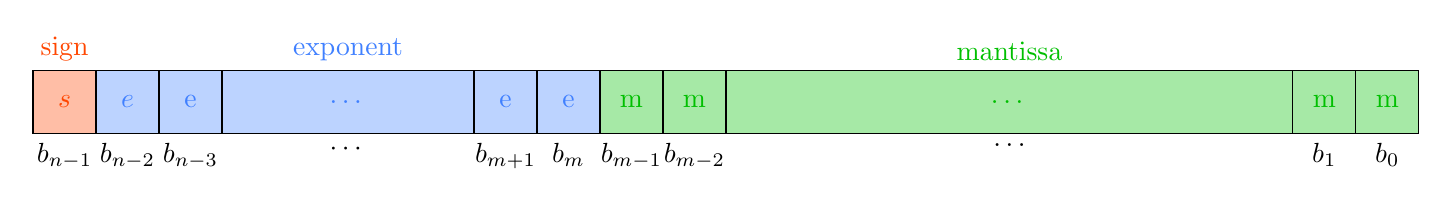
\begin{tikzpicture}


\coordinate (p);
\foreach \labela/\labelb/\inline/\c/\width in {
	\textcolor{corange}{sign}/$b_{n-1}$/$s$/corange/1,
	/$b_{n-2}$/$e$/cblue/1,
	/$b_{n-3}$/e/cblue/1,
	\textcolor{cblue}{exponent}/$\cdots$/$\dots$/cblue/4,
	/$b_{m+1}$/e/cblue/1,
	/$b_{m}$/e/cblue/1,
	/$b_{m-1}$/m/cgreen/1,
	/$b_{m-2}$/m/cgreen/1,
	\textcolor{cgreen}{mantissa}/$\ldots$/$\dots$/cgreen/9,
	/$b_1$/m/cgreen/1,
	/$b_0$/m/cgreen/1
}{
    \node[draw,fill=\c!35,minimum height=8 mm,minimum width=\width*8 mm,anchor=west,outer sep=0pt,label=below:\labelb,label=above:\labela]
    (n) at (p) {\textcolor{\c}{\inline}};
    %\draw[thick] ([yshift=-1mm]n.south west) -- ([yshift=1mm]n.north west);
    \coordinate (p) at (n.east);
}

\end{tikzpicture}


\end{document}